\documentclass{article}

\usepackage{graphicx}
\usepackage{tikz}
\usepackage{tikzsymbols}
\usetikzlibrary{calc,patterns,shapes.geometric}
\pagestyle{empty}
\usepackage[margin=0pt]{geometry}
\geometry{papersize={14in,12in}}

\def\centerarc[#1](#2)(#3:#4:#5){\draw[#1] ($(#2)+({#5*cos(#3)},{#5*sin(#3)})$) arc (#3:#4:#5);}

\begin{document}
	\begin{figure}
		\centering
		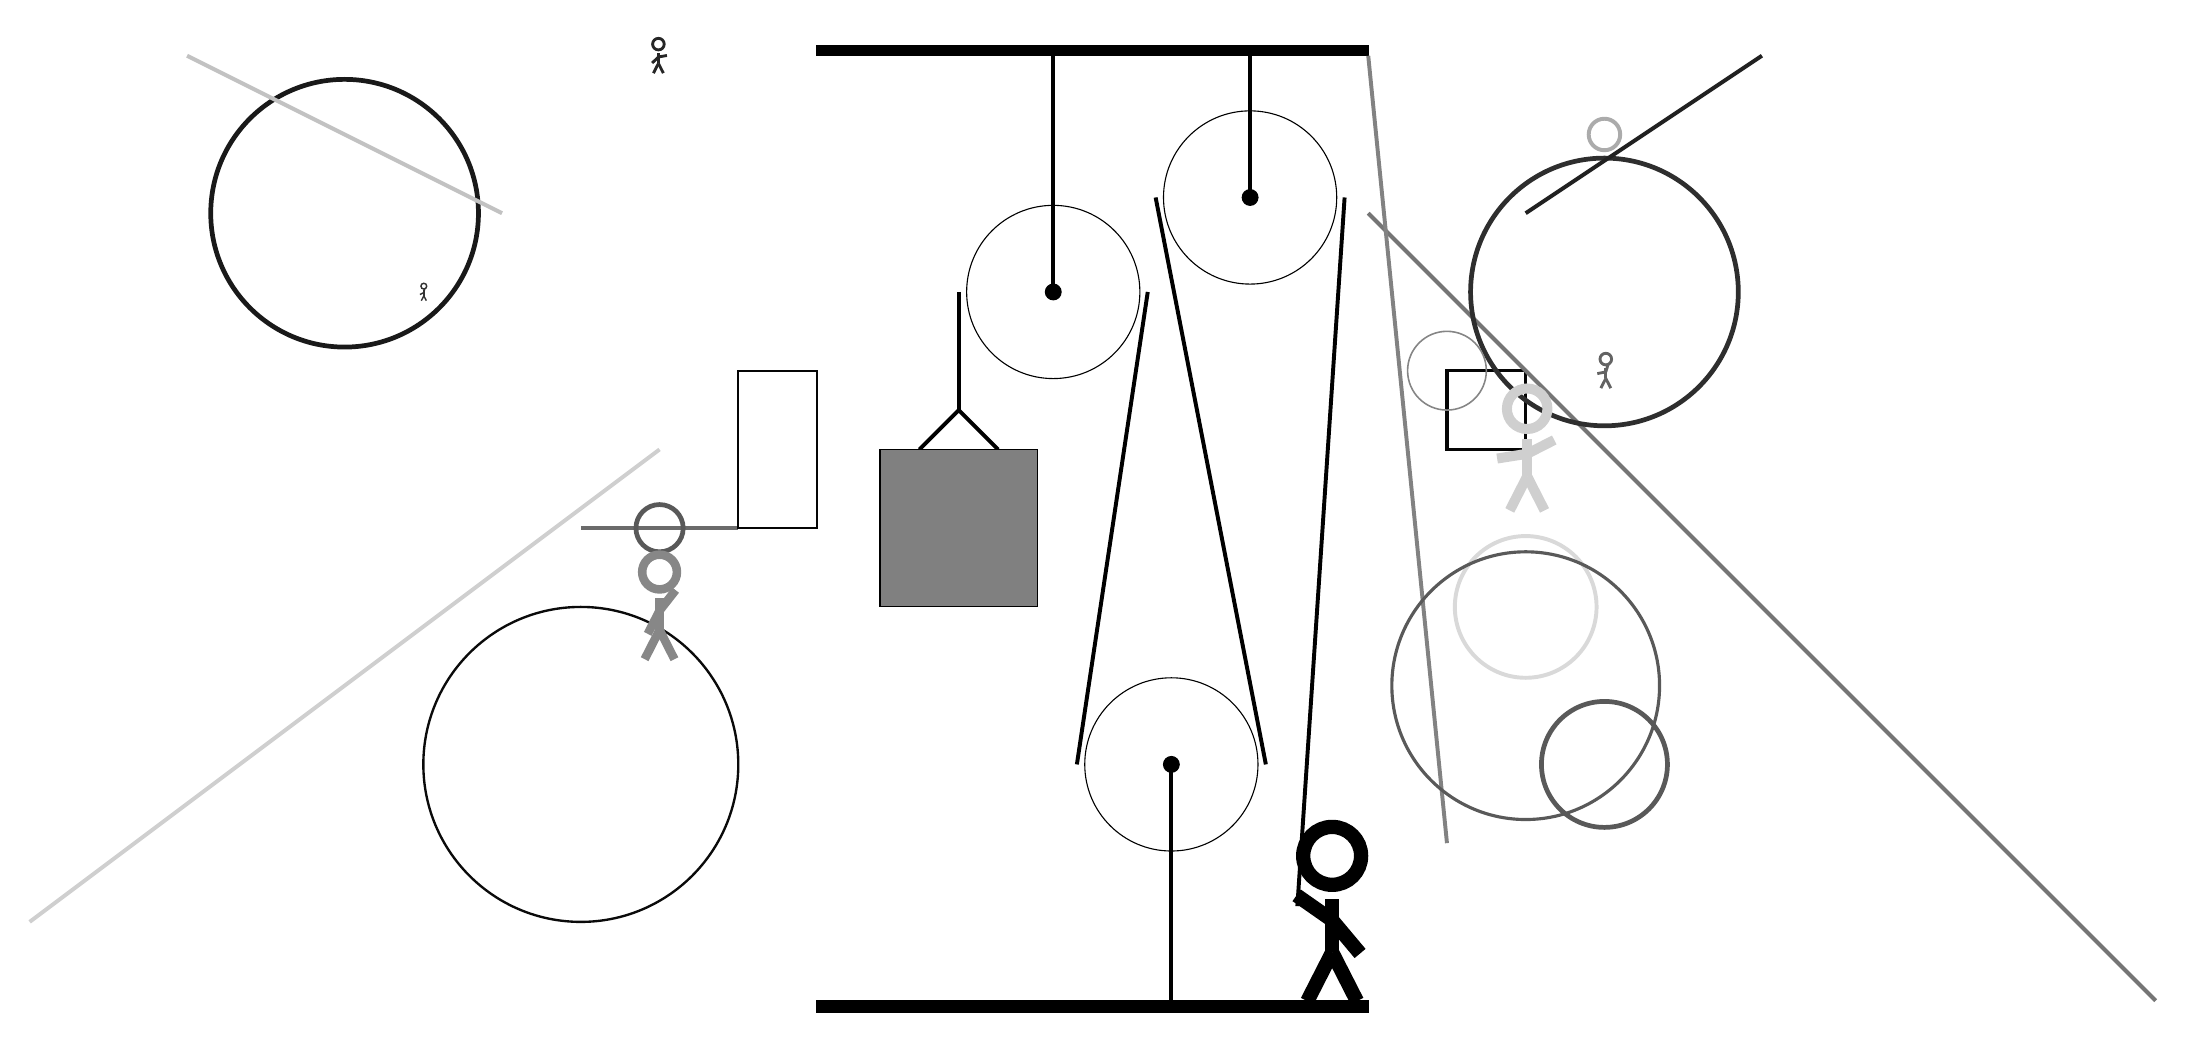
\begin{tikzpicture}
			%%%%% START %%%%%
			
			\draw[fill=black] (-2, 9) rectangle (5, 9.125);
			
			\draw (1, 6) circle (1.1);
			\draw[fill=black] (1, 6) circle (0.1);
			\draw[line width=0.5mm]  (1, 9) -- (1, 6);
			
			\draw[fill=white](2.5, 0) circle (1.1);
			\draw[fill=black] (2.5, 0) circle (0.1);
			\draw[line width=0.5mm]  (2.5, -3) -- (2.5, 0);
			
			\draw[line width=0.4mm, color=black!98] (7, 4) rectangle (6, 5);
			
			\draw[line width=0.5mm, color=black!58](-5, 3) -- (-3, 3);
			\draw[line width=0.5mm, color=black!54](5, 7) -- (15, -3);
			\node[line width=0.2mm, color=black!85] at (-4, 9) {\Strichmaxerl[2][44][10]};
			\draw [line width=0.6mm, color=black!90](-8, 7) circle (1.7);
			\node[line width=0.2mm, color=black!80] at (-7, 6) {\Strichmaxerl[1][27][77]};
			
			\draw [line width=0.5mm, color=black!33](8, 8) circle (0.2);
			\node[line width=0.5mm, color=black!61] at (8, 5) {\Strichmaxerl[2][11][73]};
			\draw [line width=0.5mm, color=black!15](7, 2) circle (0.9);
			\draw [line width=0.6mm, color=black!82](8, 6) circle (1.7);
			
			\draw [line width=0.2mm, color=black!48](6, 5) circle (0.5);
			\draw[line width=0.5mm, color=black!49](5, 9) -- (6, -1);
			\draw[line width=0.5mm, color=black!19](-4, 4) -- (-12, -2);
			
			\draw [line width=0.6mm, color=black!65](8, 0) circle (0.8);
			\draw[line width=0.5mm, color=black!24](-6, 7) -- (-10, 9);
			\draw [line width=0.6mm, color=black!65](-4, 3) circle (0.3);
			
			\node[line width=0.7mm, color=black!19] at (7, 4) {\Strichmaxerl[7][9][27]};
			\draw[line width=0.3mm, color=black!98] (-2, 3) rectangle (-3, 5);
			\draw[line width=0.5mm, color=black!87](7, 7) -- (10, 9);
			
			\draw [line width=0.3mm, color=black!96](-5, 0) circle (2.0);
			\node[line width=0.7mm, color=black!47] at (-4, 2) {\Strichmaxerl[6][63][52]};
			
			\draw [line width=0.4mm, color=black!65](7, 1) circle (1.7);
			
			\draw[fill=white](3.5, 7.2) circle (1.1);
			\draw[fill=black] (3.5, 7.2) circle (0.1);
			\draw[line width=0.5mm] (3.5, 9) -- (3.5, 7.2);
			
			\draw[line width=0.5mm] (-0.7, 4.0) -- (-0.2, 4.5) -- (0.3, 4.0);
			\draw[fill=black!50] (-1.2, 4.0) rectangle (0.8, 2.0);
			
			\draw[line width=0.5mm] (-0.2, 6) -- (-0.2, 4.5);
			\centerarc[line width=0.5mm](1, 6)(0:180:1.2000000000000002);
			\draw[line width=0.5mm](2.2, 6) -- (1.3, 0);
			\centerarc[line width=0.5mm](2.5, 0)(180:360:1.2000000000000002);
			\draw[line width=0.5mm](3.7, 0) -- (2.3, 7.2);
			\centerarc[line width=0.5mm](3.5, 7.2)(0:180:1.2000000000000002);
			\draw[line width=0.5mm](4.7, 7.2) -- (4.1, -1.8);
			
			\node at (4.5, -1.9) {\Strichmaxerl[10][-35][-50]};
			
			\draw[fill=black] (-2, -3) rectangle (5, -3.15);
			
			%%%%% END %%%%%
		\end{tikzpicture}
	\end{figure}	
\end{document}